\section{Alternative Calibration}
In this section we show results from an alternative parameter specification. Specifically, we assume that $\rho^a = 0.001$ and $\rho^b = 0.05$. 

\begin{figure}[htbp]
\centering
\vspace{0.1in}
\begin{tabular}{cc}
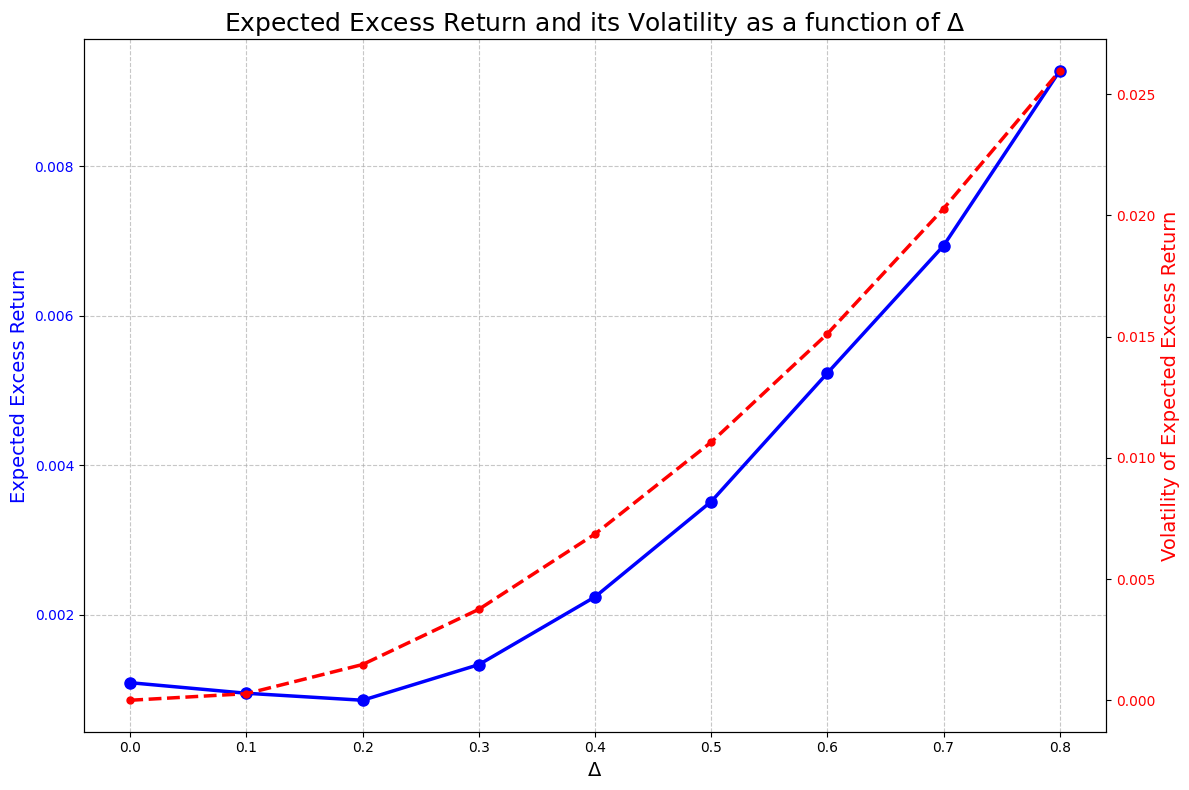
\includegraphics[width=.4\textwidth]{figures/APUnconditionalExcessReturnsJFEALT.png} &
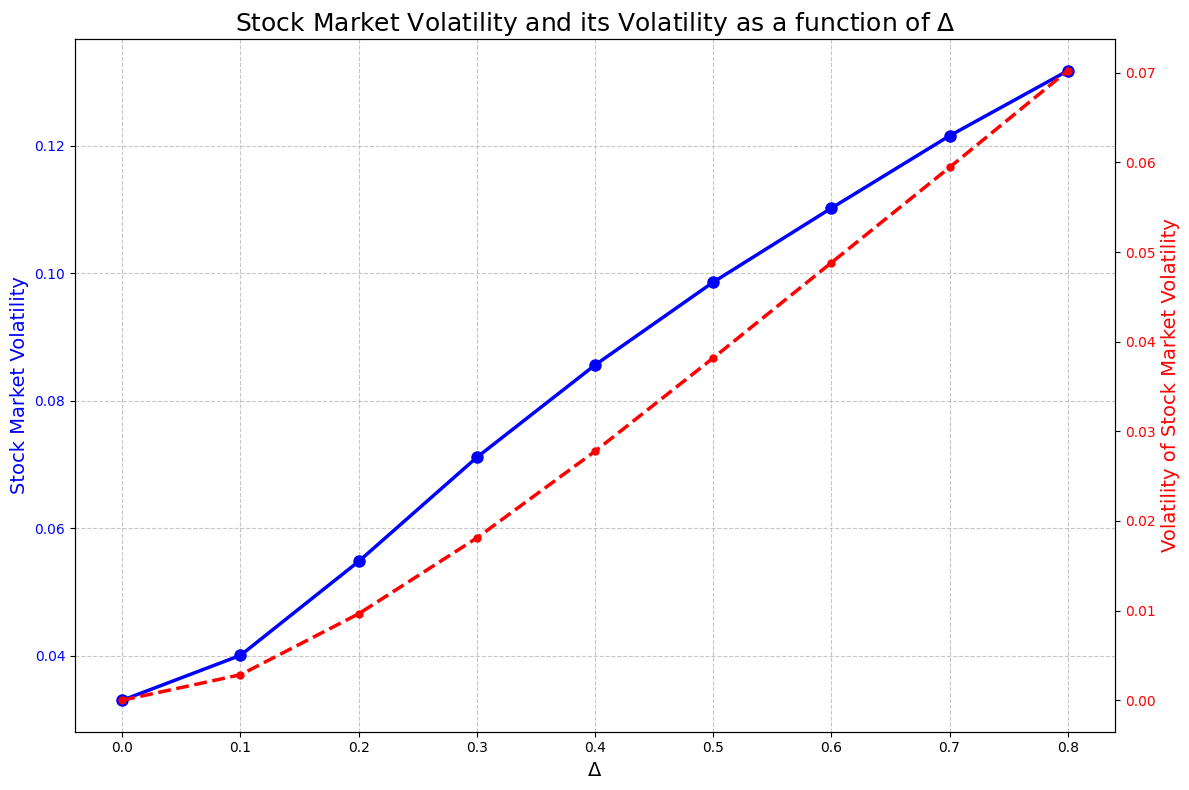
\includegraphics[width=.4\textwidth]{figures/APUnconditionalStockMarketVolatilityJFEALT.png} \\
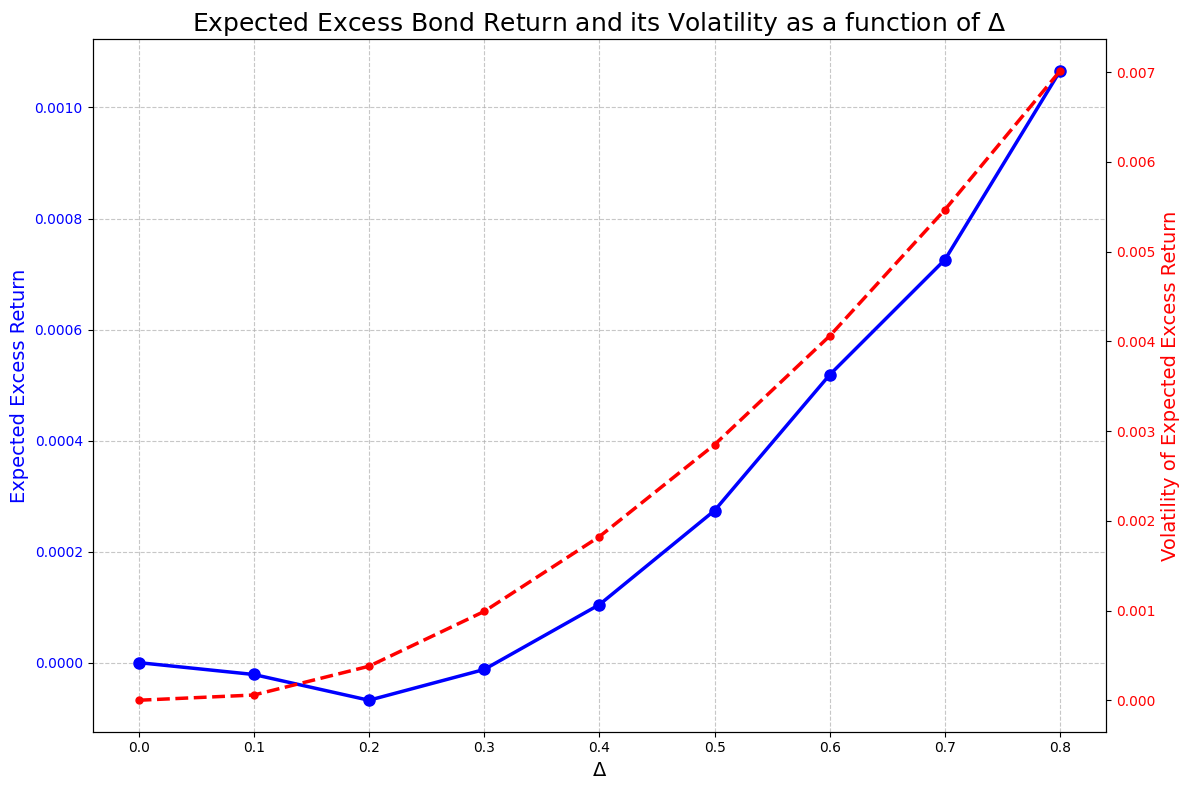
\includegraphics[width=.4\textwidth]{figures/ExRBond5yearJFEALT.png} &
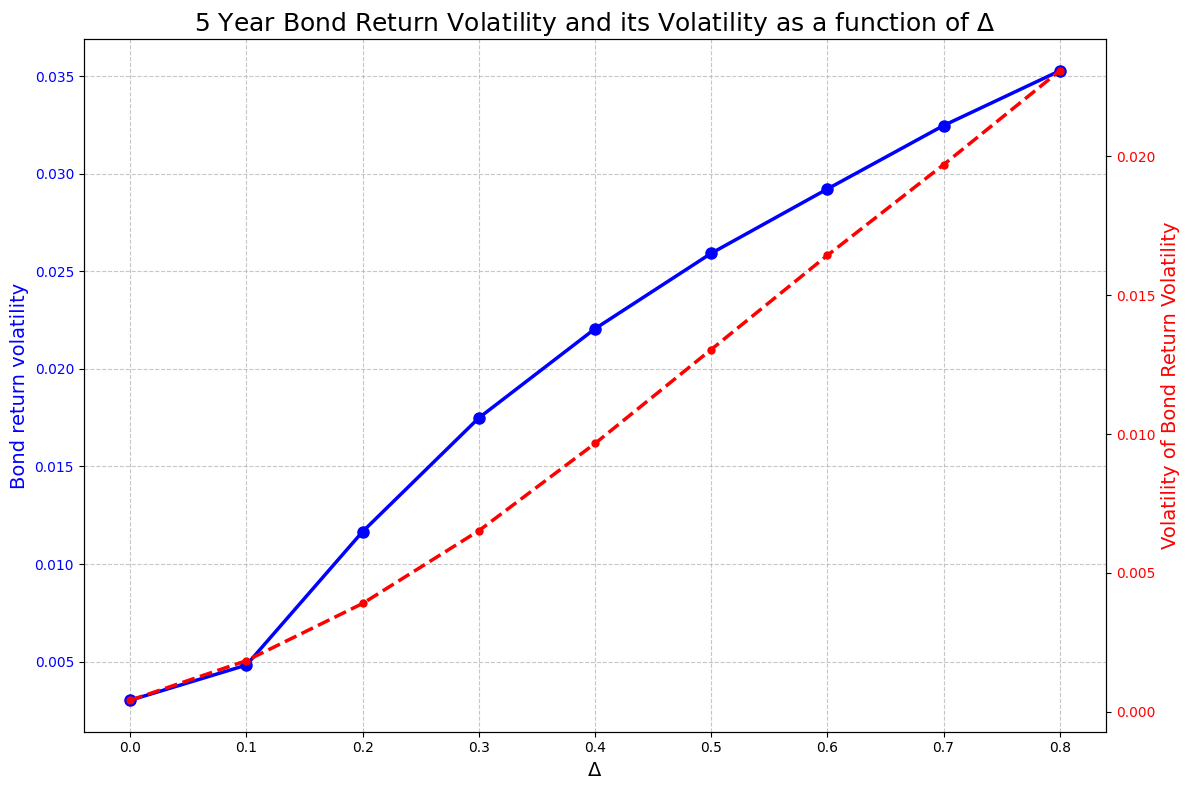
\includegraphics[width=.4\textwidth]{figures/BondVola5yearJFEALT.png} \\
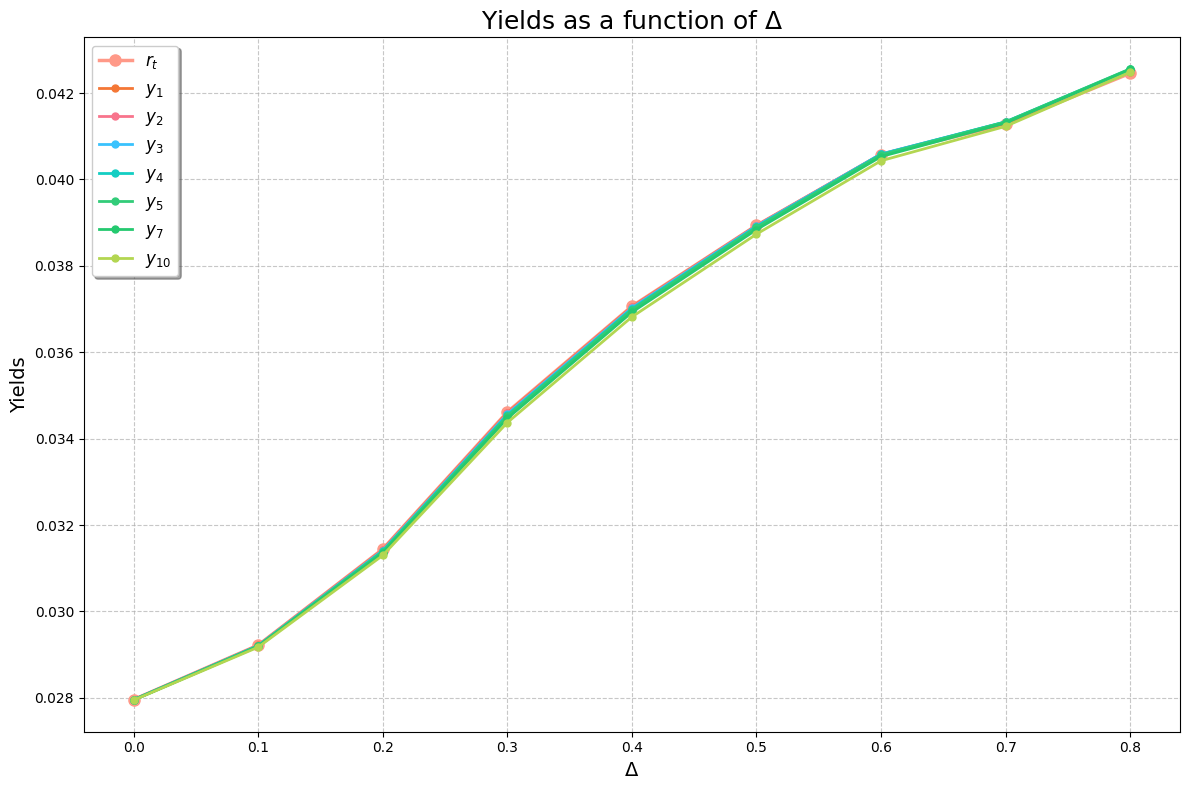
\includegraphics[width=.4\textwidth]{figures/UnconditionalYieldsJFEALT.png} &
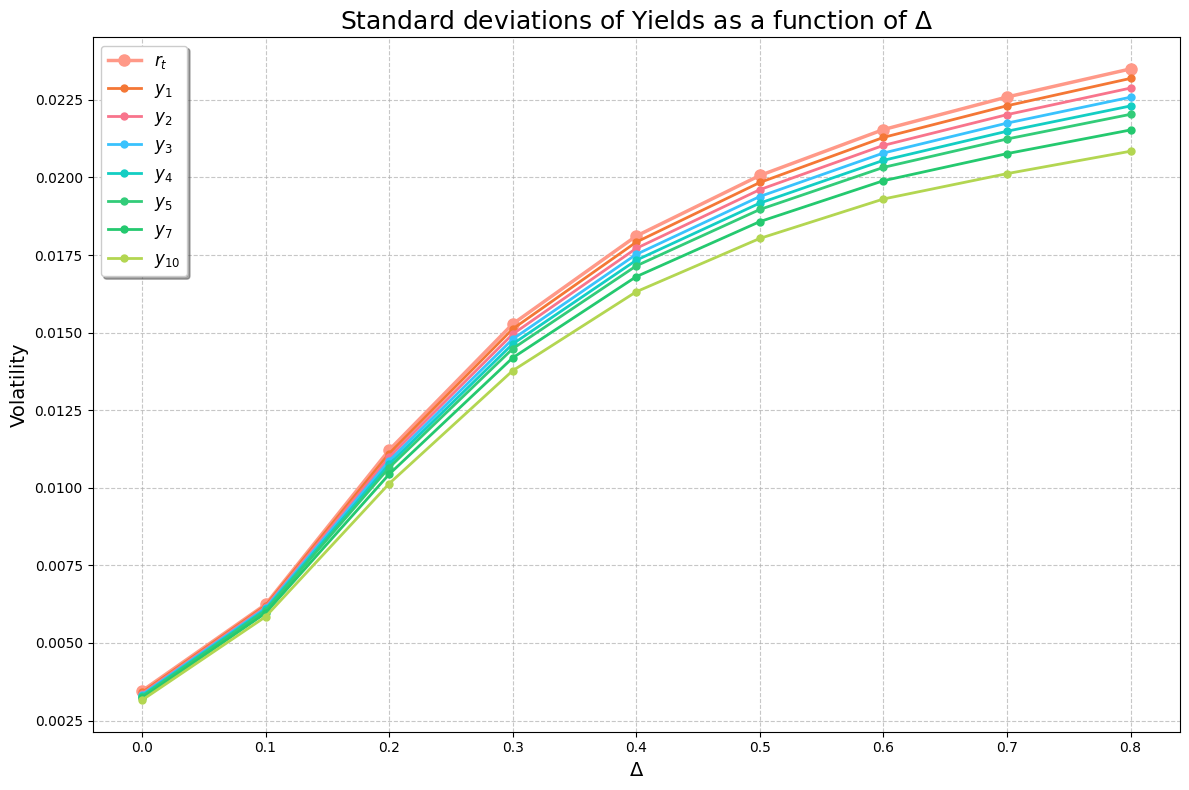
\includegraphics[width=.4\textwidth]{figures/UnconditionalYieldVolatilitiesJFEALT.png} \\ 
\end{tabular}
\caption{\textbf{Unconditional Asset Pricing Moments.} \footnotesize{The figures show the expected excess stock market return (top-left), stock market volatility (top-right), excess return on the five year bond (middle-left), the standard deviation of the five year bond return (middle-right), the yield curve  (bottom left} and the volatility of yields (bottom right).}  \label{fig:UnconditionalAPALT} 
\end{figure}

\begin{figure}[htbp]
\centering
\vspace{0.1in}
\begin{tabular}{cc}
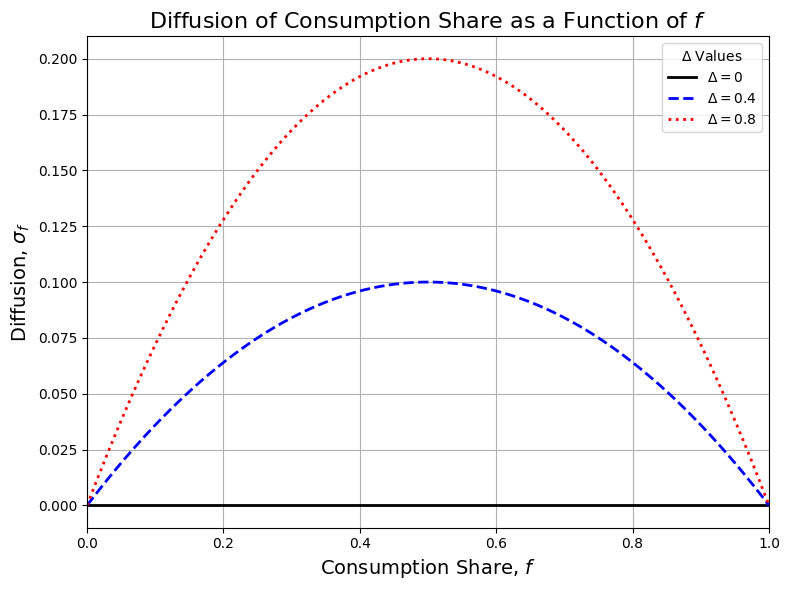
\includegraphics[width=.3\textwidth]{figures/sigfALT.png} &
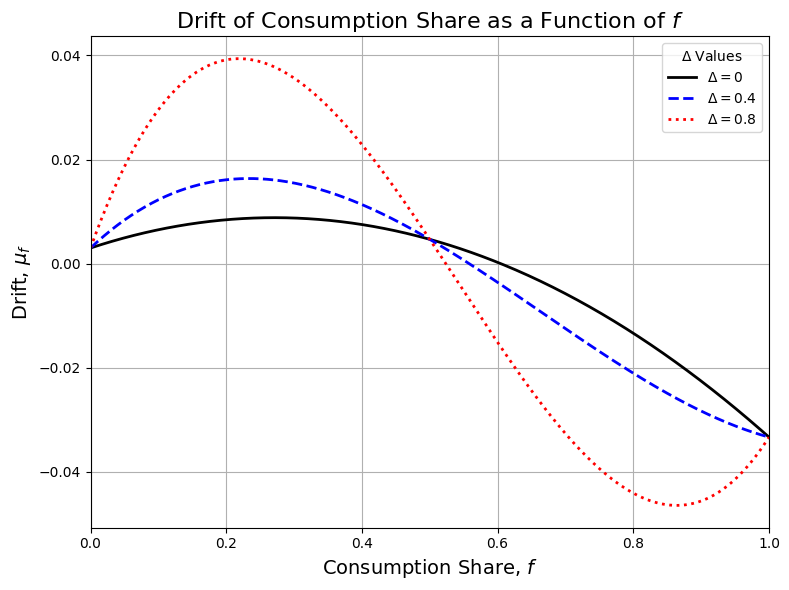
\includegraphics[width=.3\textwidth]{figures/mufALT.png} \\
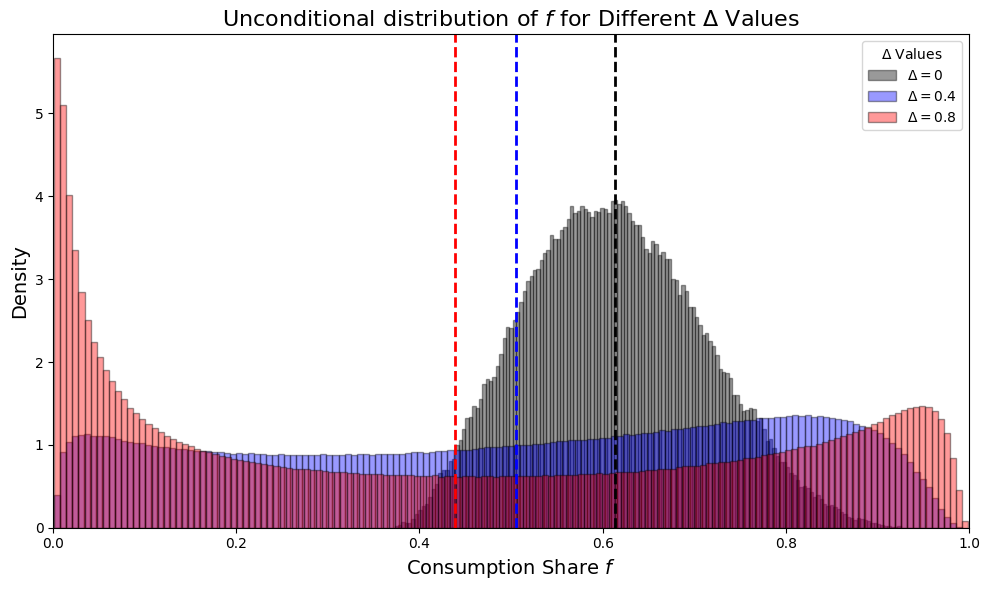
\includegraphics[width=.3\textwidth]{figures/distfALT.png} &
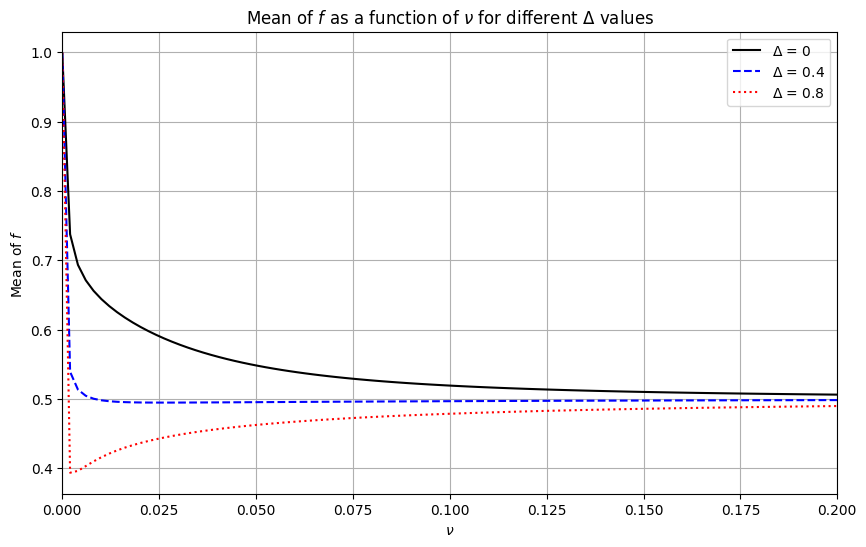
\includegraphics[width=.3\textwidth]{figures/meanfasnuALT.png}
\end{tabular}
\caption{\textbf{The consumption share.} \footnotesize{The top left graph shows the volatility $\sigma_{f,t}$ and the top right graph shows the drift $\mu_{f,t}$ of the consumption share dynamics as a function of the consumption share for three levels of disagreement $\Delta$. The drift of the consumption share $\mu_{f,t}$ in the top right graph depends on the fraction of patient newborns $\alpha_t$ which is fixed at 0.5. The left graph shows the unconditional distribution of the consumption share of patient investors $\tilde{f}$ and the right graph shows the unconditional mean of the consumption share of patient investors $\mathrm{E}[\tilde{f}]$ as a function of the birth/mortality rate $\nu$. The histograms and unconditional means in the bottom row are based 500K years of monthly observations for each value of disagreement $\Delta$.}} \label{fig:ConsumptionShareALT} 
\end{figure}

\begin{figure}[htbp]
\centering
\vspace{0.1in}
\begin{tabular}{cc}
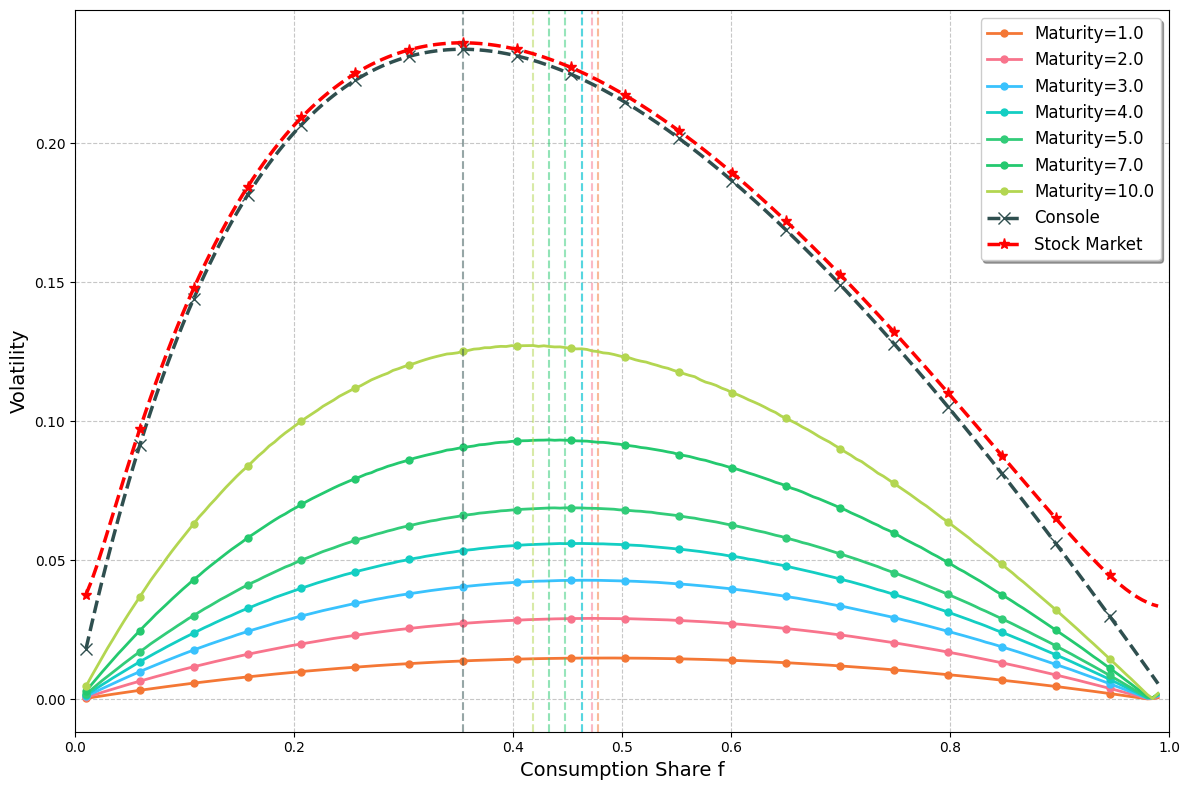
\includegraphics[width=.45\textwidth]{figures/volAPV3ALT.png} &
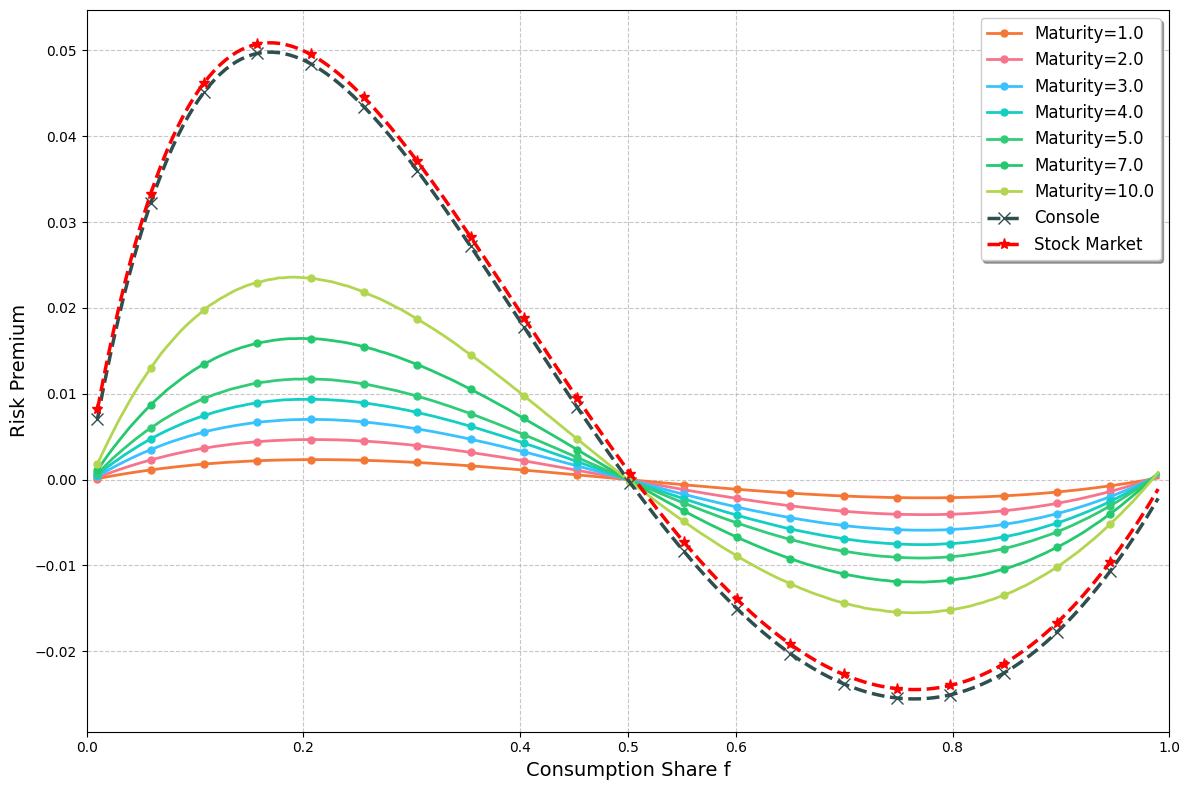
\includegraphics[width=.45\textwidth]{figures/RPV3ALT.png}
\end{tabular}
\caption{\textbf{Conditional Return volatility and risk premium of bonds and stocks.} \footnotesize{The left graph shows bond return volatility and the right graphs shows the bond risk premium as a function of the consumption share $f_t$ for different maturities. In all figures we keep $\alpha = 0.5$.}} \label{fig:VolaRiskPremium2fALT} 
 \end{figure}
